\chapter{Stamcellen, regeneratie en veroudering}\label{ch:b3:stem-cells}

Snijd een axolotl een poot af en binnen twee maanden heeft hij een
nieuwe laten groeien, met bot, spier, zenuw en huid op de juiste
plaatsen, en hij doet het telkens opnieuw, hoe vaak er ook wordt
gesneden. Snijd een planarie in twintig stukken en elk wordt binnen
veertien dagen een hele worm, waarbij het stuk dat een staart was een
kop met ogen en een brein laat teruggroeien. Snijd een mens een vinger
af boven het laatste kootje en die geneest als een litteken. Toch is het
menselijke lichaam niet zonder vernieuwing: elke seconde maakt het twee
miljoen rode bloedcellen, de bekleding van de darm wordt om de vijf
dagen vervangen en de huid elke maand, en dat alles stamt af van kleine
groepen cellen die zich een leven lang delen zonder zichzelf uit te
putten. Dit hoofdstuk gaat over die cellen --- wat een \omterm{def:b3:stem-cells:stem}{stamcel} tot
\omterm{def:b3:stem-cells:stem}{stamcel} maakt, hoe haar \omterm{def:b3:stem-cells:stem}{nis} haar zo houdt, hoe de hele hiërarchie van
bloed of darm eruit wordt opgebouwd --- over de dieren die kunnen laten
teruggroeien wat de mens niet kan en waarom, over de ontdekking dat elke
cel met vier genen naar de embryonale toestand kan worden teruggeduwd,
en over wat de rekenkunde van de celdeling te zeggen heeft over waarom
de mens veroudert.

\section{Wat een stamcel is}

\begin{definition}[Stamcellen en hun hiërarchie]\label{def:b3:stem-cells:stem}
\index{stamcel}\index{zelfvernieuwing}\index{asymmetrische deling}\index{voorlopercel}\index{doorgangsversterkende cel}\index{nis}
Een \emph{stamcel} heeft twee kenmerkende eigenschappen: zij kan
\emph{zichzelf vernieuwen} en dochters voortbrengen die stamcel zijn,
en zij kan dochters voortbrengen die differentiëren. Zij kan beide
tegelijk doen, door een \emph{asymmetrische deling} met van elke soort
één dochter, waarbij het lot wordt bepaald door een ongelijke
overerving van determinanten of door welke dochter in contact blijft
met de \emph{nis} --- de omgeving van naburige cellen, matrix en
signalen die een cel stamcel houdt; of zij kan symmetrisch delen,
waarbij sommige delingen twee stamcellen en andere twee differentiërende
cellen opleveren, met een populatie die gemiddeld constant blijft. De
differentiërende dochters doorlopen gewoonlijk stadia van
\emph{voorlopercel} of \emph{doorgangsversterking}, waarin zij nog
enkele malen delen met een steeds nauwere potentie voordat zij rijpen:
de hiërarchie versterkt enkele trage delingen van stamcellen tot een
grote opbrengst, en beperkt het aantal delingen dat een stamcel moet
maken. Stamcellen van de volwassene zijn zeldzaam en traag --- een
bloedvormende stamcel deelt misschien eens per jaar, een stamcel van de
darm eens per dag --- en \emph{multipotent}, beperkt tot de lijnen van
hun eigen weefsel; embryonale stamcellen, uit de binnenste celmassa van
de blastocyste, zijn \emph{pluripotent} en kunnen elk weefsel van het
lichaam maken maar niet de placenta.
\end{definition}

\begin{omfigure}
\begin{tikzpicture}[every node/.style={font=\scriptsize}, >=stealth]
  \node[draw, very thick, rounded corners, fill=omDef!25, align=center] (hsc) at (0,3.6) {bloedvormende stamcel\\$\sim$\num{10000} bij een mens; deelt $\sim$ eens per jaar};
  \node[draw, thick, rounded corners, fill=omDef!12, align=center] (mpp) at (0,2.4) {multipotente voorlopercellen};
  \node[draw, thick, rounded corners, fill=omThm!15, align=center] (cmp) at (-3.2,1.2) {myeloïde voorlopercel};
  \node[draw, thick, rounded corners, fill=omProp!20, align=center] (clp) at (3.2,1.2) {lymfoïde voorlopercel};
  \node[align=center, font=\tiny] (e) at (-5.4,-0.4) {erytrocyten\\$2\times 10^{11}$/dag};
  \node[align=center, font=\tiny] (pl) at (-3.6,-0.4) {bloedplaatjes\\(megakaryocyten)};
  \node[align=center, font=\tiny] (g) at (-1.8,-0.4) {granulocyten\\$10^{11}$/dag};
  \node[align=center, font=\tiny] (m) at (-0.2,-0.4) {monocyten,\\macrofagen};
  \node[align=center, font=\tiny] (b) at (1.8,-0.4) {B-cellen};
  \node[align=center, font=\tiny] (t) at (3.4,-0.4) {T-cellen};
  \node[align=center, font=\tiny] (nk) at (5.0,-0.4) {NK-cellen};
  \draw[->, thick] (hsc) -- (mpp); \draw[->, thick] (mpp) -- (cmp); \draw[->, thick] (mpp) -- (clp);
  \foreach \x in {e,pl,g,m} { \draw[->, thick] (cmp) -- (\x); }
  \foreach \x in {b,t,nk} { \draw[->, thick] (clp) -- (\x); }
  \draw[->, thick, omDef!70!black] (hsc.west) .. controls (-3.0,4.4) and (-3.0,3.0) .. (hsc.south west) node[pos=0.5, left, font=\tiny, omDef!70!black, align=right] {zelfvernieuwing};
  \node[right, align=left, font=\tiny] at (4.4,3.6) {elke laag deelt vaker\\en heeft een nauwere potentie;\\$\sim 20$ delingen van stamcel\\tot rode cel, zodat één deling\\van een stamcel $\sim 10^{6}$ cellen oplevert};
\end{tikzpicture}

{\small De hiërarchie van de bloedvorming. Enkele duizenden trage
\omterm{def:b3:stem-cells:stem}{stamcellen} in het merg voeden \omterm{def:b3:stem-cells:stem}{voorlopercellen} die snel delen en zich
stap voor stap vastleggen, zodat de opbrengst van een biljoen cellen
per dag de \omterm{def:b3:stem-cells:stem}{stamcellen} bijna niets kost.}
\end{omfigure}

\begin{proof}[Bewijsmateriaal]
Till en McCulloch (1961) spoten mergcellen in dodelijk bestraalde
muizen en telden de knobbeltjes die tien dagen later op de milt
verschenen: elk was een kolonie bloedcellen van verscheidene lijnen,
hun aantal evenredig met het aantal ingespoten cellen, en het merken
van de chromosomen van de donorcellen toonde dat elke kolonie een kloon
was --- één cel had rode cellen, granulocyten en bloedplaatjes gemaakt,
en sommige kolonies bevatten cellen die in een tweede muis nieuwe
kolonies konden zaaien: \omterm{def:b3:stem-cells:stem}{zelfvernieuwing} en multipotentie in één cel, de
werkbare definitie van een \omterm{def:b3:stem-cells:stem}{stamcel} en de grondslag van de
beenmergtransplantatie. Barker en Clevers (2007) merkten cellen die het
gen \emph{Lgr5} tot expressie brengen aan de basis van darmcrypten met
een erfelijke kleur en zagen die kleur in de loop van weken de crypte
opklimmen en hele villi vullen: de gemerkte cellen waren de \omterm{def:b3:stem-cells:stem}{stamcellen}
van de darm, en één ervan, gekweekt in een gel met de juiste drie
groeifactoren, groeide uit tot een darm in het klein, een
\emph{\omterm{def:b3:stem-cells:pluripotency}{organoïde}}, met eigen crypten en villi (Sato, 2009).
\end{proof}

\begin{proposition}[De nis en de crypte]\label{prop:b3:stem-cells:crypt}
\index{crypte}\index{Lgr5}\index{Panethcel}\index{Wnt-signalering}\index{neutrale drift}
De \emph{crypte} van de darm is de best begrepen \omterm{def:b3:stem-cells:stem}{nis}. Aan haar basis
zitten ongeveer veertien \emph{Lgr5}-stamcellen ingeklemd tussen
\omterm{prop:b3:stem-cells:crypt}{Panethcellen}, die de signalen van Wnt en Notch en de groeifactoren
uitscheiden die hen \omterm{def:b3:stem-cells:stem}{stamcel} houden; een \omterm{def:b3:stem-cells:stem}{stamcel} die omhoog wordt geduwd
en het contact met de \omterm{prop:b3:stem-cells:crypt}{Panethcellen} verliest, mist het signaal binnen
enkele celdiameters en wordt een \omterm{def:b3:stem-cells:stem}{doorgangsversterkende cel}, die in de
crypte vier of vijf maal deelt en daarna differentieert tot de
opnemende en uitscheidende cellen die de villus op trekken en vijf
dagen later van de punt worden afgestoten. De \omterm{def:b3:stem-cells:stem}{stamcellen} delen
symmetrisch, ongeveer eens per dag, en wedijveren om de beperkte ruimte
in de \omterm{def:b3:stem-cells:stem}{nis}: bij toeval breidt één kloon zich uit en gaan de andere
verloren, zodat binnen enkele maanden elke crypte van één \omterm{def:b3:stem-cells:stem}{stamcel}
afstamt --- de \emph{\omterm{prop:b3:stem-cells:crypt}{neutrale drift}} op de schaal van een crypte, een
toevalswandeling met absorberende randen. De \omterm{def:b3:stem-cells:stem}{nis}, niet de cel, draagt
de stamcelaard: zet een gedifferentieerde cel na een verwonding weer in
contact met de signalen van de \omterm{prop:b3:stem-cells:crypt}{Panethcellen} en zij kan terugkeren; haal
de \omterm{def:b3:stem-cells:stem}{stamcel} eruit en geef haar de signalen in een schaaltje en zij maakt
een \omterm{def:b3:stem-cells:pluripotency}{organoïde}. Beenmerg, haarzakjes, de teelbal en de zones met neurale
\omterm{def:b3:stem-cells:stem}{stamcellen} in het brein volgen dezelfde logica met andere signalen.
\end{proposition}
\begin{proof}[Bewijsmateriaal]
Snippert en collega's (2010) merkten de \omterm{def:b3:stem-cells:stem}{stamcellen} van crypten met een
``confetti'' van vier willekeurige kleuren; de crypten waren
aanvankelijk veelkleurig en waren na enkele maanden eenkleurig
geworden, met een tempo dat past bij symmetrische deling en neutrale
mededinging tussen ongeveer veertien cellen --- en niet bij
\omterm{def:b3:stem-cells:stem}{asymmetrische deling}, die elke kleur onbeperkt zou hebben behouden. De
\omterm{prop:b3:stem-cells:crypt}{Panethcellen} weghalen doet de voorraad \omterm{def:b3:stem-cells:stem}{stamcellen} krimpen; het
Wnt-signaal weghalen leegt de crypte binnen dagen.
\end{proof}

\begin{omfigure}
\begin{tikzpicture}[every node/.style={font=\scriptsize}, >=stealth]
  % crypt-villus
  \draw[very thick, omDef] (0,-2.6) .. controls (0,-0.4) and (0.4,0) .. (0.8,0) -- (0.8,3.6) .. controls (0.8,4.1) and (1.6,4.1) .. (1.6,3.6) -- (1.6,0) .. controls (2.0,0) and (2.4,-0.4) .. (2.4,-2.6);
  \draw[very thick, omDef] (0,-2.6) arc[start angle=180, end angle=360, radius=1.2];
  % stem cells at base
  \foreach \a in {200,230,260,290,320} { \fill[omThm!60] ({1.2+1.05*cos(\a)},{-2.6+1.05*sin(\a)}) circle (0.14); }
  \foreach \a in {215,245,275,305} { \fill[omMeth!60] ({1.2+0.75*cos(\a)},{-2.6+0.75*sin(\a)}) circle (0.13); }
  \node[right, align=left, font=\tiny] at (2.6,-3.4) {basis: $\sim 14$ \emph{Lgr5}-stamcellen (rood)\\ingeklemd tussen Panethcellen (groen),\\die Wnt, Notch en EGF leveren};
  % TA zone
  \foreach \y in {-1.8,-1.3,-0.8,-0.3} { \fill[omProp!50] (0.35,\y) circle (0.11); \fill[omProp!50] (2.05,\y) circle (0.11); }
  \node[right, align=left, font=\tiny] at (2.6,-1.1) {doorgangsversterkende zone:\\4--5 delingen, één per dag,\\buiten bereik van de Panethsignalen};
  % villus cells
  \foreach \y in {0.4,1.0,1.6,2.2,2.8} { \fill[omDef!40] (0.95,\y) circle (0.1); \fill[omDef!40] (1.45,\y) circle (0.1); }
  \node[right, align=left, font=\tiny] at (2.6,1.8) {villus: gedifferentieerde cellen\\trekken omhoog en worden na\\$\sim 5$ dagen van de punt afgestoten};
  \node[left, font=\tiny] at (-0.1,-2.6) {crypte}; \node[left, font=\tiny] at (0.7,3.9) {punt van de villus};
  % confetti panel
  \begin{scope}[shift={(8.8,0.2)}]
    \node[above, align=center] at (0,1.3) {neutrale drift in de nis};
    \foreach \i/\cols in {0/{omDef!60,omThm!60,omMeth!60,omProp!60,omDef!60,omThm!60}, 1/{omDef!60,omDef!60,omThm!60,omThm!60,omThm!60,omProp!60}, 2/{omThm!60,omThm!60,omThm!60,omThm!60,omDef!60,omThm!60}, 3/{omThm!60,omThm!60,omThm!60,omThm!60,omThm!60,omThm!60}} {
      \foreach [count=\j] \c in \cols { \fill[\c] ({\j*0.36-1.26},{1.0-\i*0.7}) circle (0.15); }
    }
    \node[left, font=\tiny] at (-1.35,1.0) {week 0}; \node[left, font=\tiny] at (-1.35,0.3) {week 4}; \node[left, font=\tiny] at (-1.35,-0.4) {week 12}; \node[left, font=\tiny] at (-1.35,-1.1) {maanden};
    \node[below, align=center, font=\tiny] at (0,-1.75) {klonen wedijveren om een vast aantal\\plaatsen; één wint bij toeval};
  \end{scope}
\end{tikzpicture}

{\small De crypte als \omterm{def:b3:stem-cells:stem}{nis}. De stamcelaard is een plaats: cellen die in
contact staan met de signalen van de \omterm{prop:b3:stem-cells:crypt}{Panethcellen} blijven \omterm{def:b3:stem-cells:stem}{stamcel},
cellen die uit dat contact worden geduwd beginnen aan de reis van vijf
dagen naar de punt van de villus. Met willekeurige kleuren gemerkt
drijven de \omterm{def:b3:stem-cells:stem}{stamcellen} van een crypte binnen maanden naar één kloon af.}
\end{omfigure}

\section{Pluripotentie en herprogrammering}

\begin{definition}[Embryonaal, geïnduceerd en gekweekt]\label{def:b3:stem-cells:pluripotency}
\index{embryonale stamcel}\index{pluripotentie}\index{geïnduceerde pluripotente stamcel}\index{herprogrammering}\index{organoïde}
\emph{Embryonale \omterm{def:b3:stem-cells:stem}{stamcellen}} (Evans, Kaufman, Martin, 1981, muis;
Thomson, 1998, mens) zijn cellen uit de binnenste celmassa die in kweek
aan het delen worden gehouden zonder te differentiëren, door signalen
(LIF, of FGF en activine) die een kern van transcriptiefactoren ---
Oct4, Sox2, Nanog --- in stand houden, die elkaar activeren en de genen
van elke lijn onderdrukken. In een blastocyste gespoten voegen zij zich
bij het embryo en dragen zij bij aan al zijn weefsels, met inbegrip van
de kiembaan, en zo wordt de knock-outmuis gemaakt: verander een gen in
de cellen en maak er een muis van. De kernoverdracht uit het deel van
het tweede jaar liet zien dat een gedifferentieerde kern door het
cytoplasma van een eicel kan worden teruggezet; Takahashi en Yamanaka
(2006) vonden wat dat terugzetten doet. Van vierentwintig
kandidaatgenen zetten er vier --- \emph{Oct4}, \emph{Sox2},
\emph{Klf4}, \emph{c-Myc} --- samen op virussen in huidfibroblasten
gebracht, in drie weken ongeveer één cel op duizend om in een
\emph{geïnduceerde pluripotente \omterm{def:b3:stem-cells:stem}{stamcel}} die niet van een embryonale te
onderscheiden is en elk weefsel en een hele muis kan vormen.
\emph{Herprogrammering} is traag en ondoelmatig omdat de factoren
\omterm{def:b3:chromatin-epigenetics:nucleosome}{chromatine} moeten openen dat door jaren van differentiatie is gesloten,
en de cellen een toevallige fase doorlopen waarin de meeste blijven
steken; zij is in beginsel ook een weg van de eigen cellen van een
patiënt naar elk weefsel. Geef de juiste signalen in de juiste volgorde
en pluripotente cellen in een schaaltje spelen de ontwikkeling na:
hartspier die klopt, dopamineneuronen om in een brein met de ziekte van
Parkinson te plaatsen, netvliescellen, en \emph{organoïden} --- zichzelf
ordenende driedimensionale weefsels van enkele millimeters, van darm,
nier, lever en hersenen, met de bouw en de celtypen van het orgaan,
waarin de menselijke ontwikkeling en ziekte kunnen worden bekeken en
geneesmiddelen kunnen worden getoetst.
\end{definition}

\begin{omfigure}
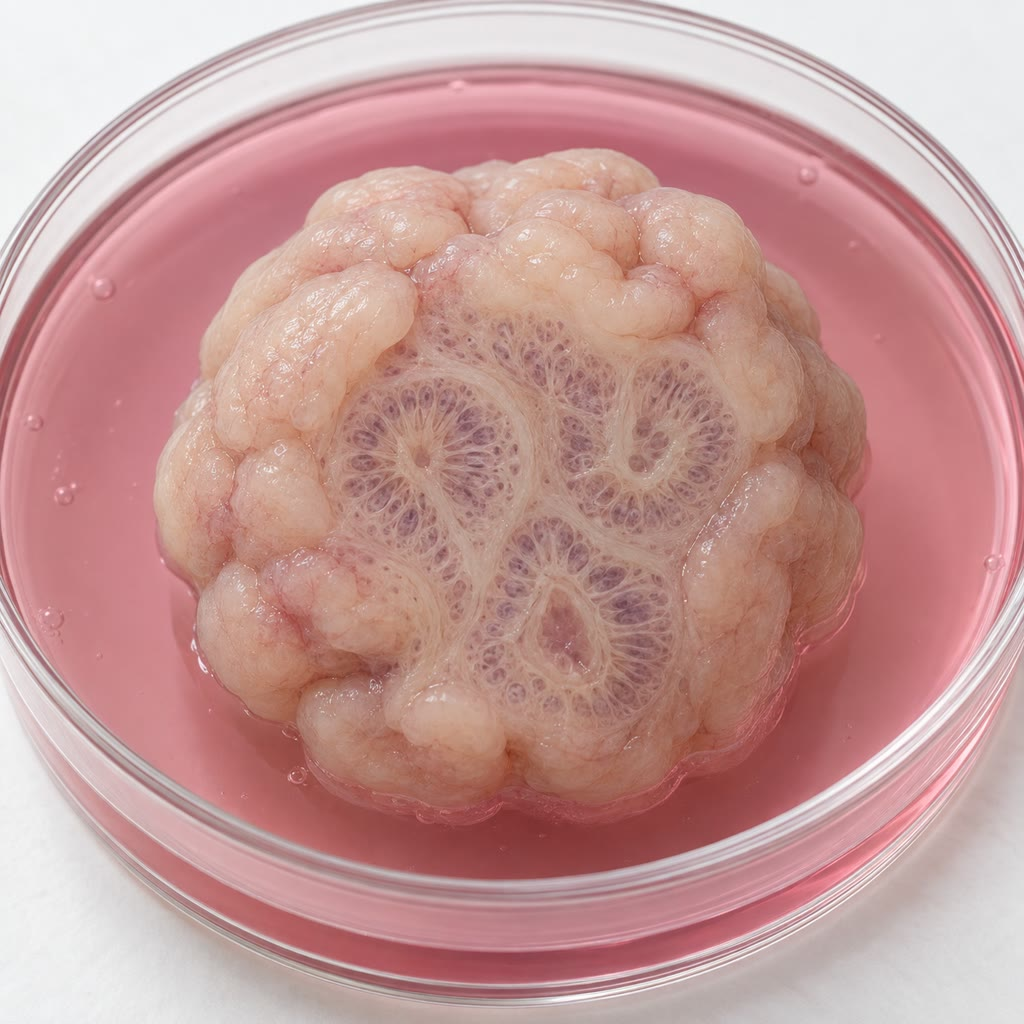
\includegraphics[width=0.4\linewidth]{images/book5/ai/b5-24-brain-organoid.jpg}\hspace{0.04\linewidth}
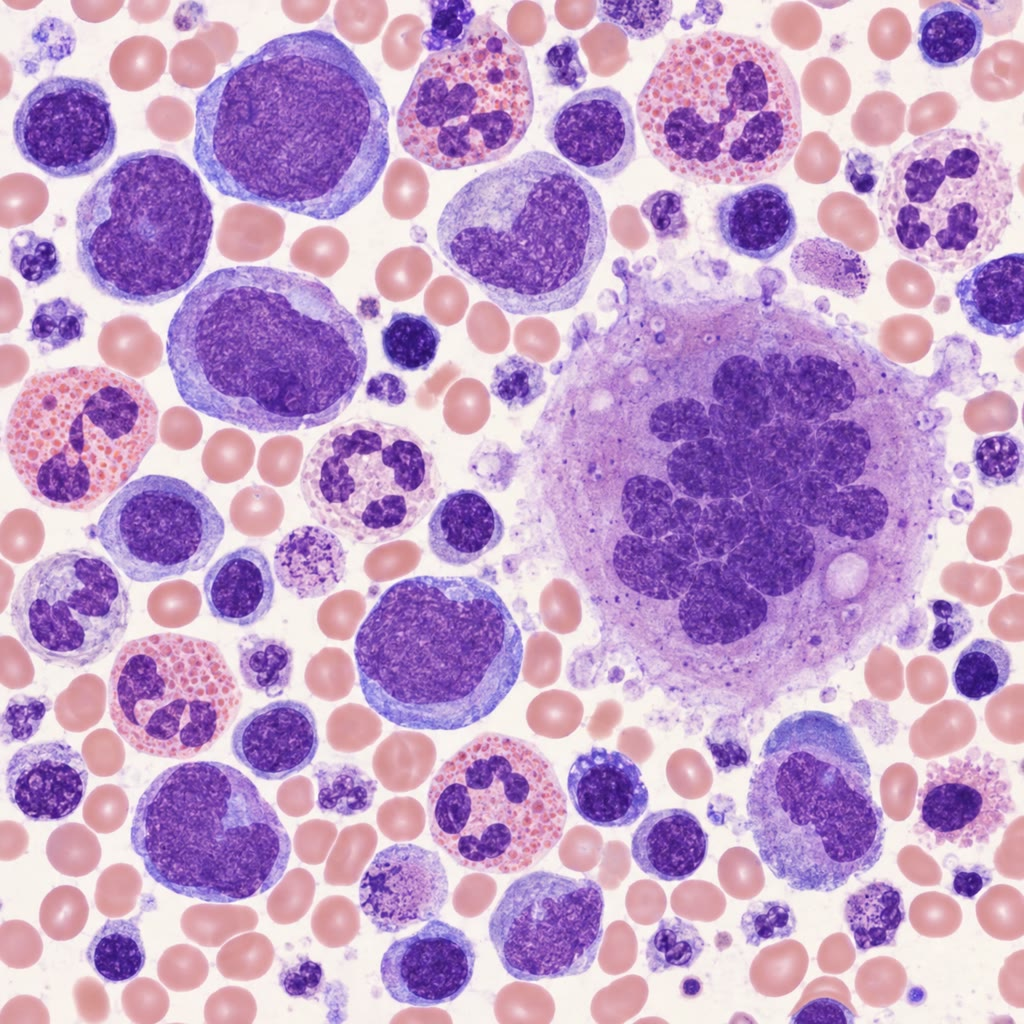
\includegraphics[width=0.4\linewidth]{images/book5/ai/b5-24-bone-marrow-smear.jpg}

{\small Links: een hersenorganoïde gekweekt uit menselijke pluripotente
cellen --- enkele millimeters zichzelf ordenend weefsel dat op schors
lijkt, met holten als ventrikels en gelaagde neuronen. Rechts: een
uitstrijkje van beenmerg, de hiërarchie van de eerste figuur in één
beeld: blasten, rijpende granulocyten, voorlopers van rode cellen en
een megakaryocyt.}
\end{omfigure}

\begin{method}[Lijnen volgen]\label{met:b3:stem-cells:tracing}
\index{lijnen volgen}\index{Cre-recombinase}
Om te vinden welke cellen de \omterm{def:b3:stem-cells:stem}{stamcellen} van een weefsel zijn: (1) kies
een gen dat door de kandidaatcellen tot expressie wordt gebracht en zet
onder zijn promotor een induceerbaar recombinase (Cre-ER, dat alleen
werkt wanneer er tamoxifen wordt gegeven); (2) breng in hetzelfde dier
een reportergen in dat blijvend actief wordt zodra het recombinase er
een stopcassette uit knipt --- een kleur die door elke nakomeling wordt
geërfd; (3) geef één dosis tamoxifen om de kandidaatcellen op één
ogenblik te merken; (4) neem met tussenpozen weefsel af en beoordeel de
gemerkte klonen: een kloon die groeit, maanden blijft bestaan en elk
celtype van het weefsel bevat komt van een \omterm{def:b3:stem-cells:stem}{stamcel}; een kloon die
binnen een week wordt afgestoten komt van een doorgangscel. (5) Volg
met een meerkleurig reportergen de mededinging tussen de klonen.
(6) Toets de functie rechtstreeks door de gemerkte cellen te doden met
een gifreceptor onder dezelfde promotor, en kijk of het weefsel zich
niet meer vernieuwt.
\end{method}

\section{Regeneratie}

\begin{definition}[Hoe dieren teruggroeien]\label{def:b3:stem-cells:regeneration}
\index{regeneratie}\index{neoblast}\index{blasteem}\index{dedifferentiatie}\index{compenserende groei}
Regeneratie verloopt langs drie wegen. \emph{Hydra} en de planarie
steunen op pluripotente \omterm{def:b3:stem-cells:stem}{stamcellen} van de volwassene: de
\emph{neoblasten} van een planarie, een vijfde van haar cellen, zijn de
enige delende cellen die zij heeft, trekken naar een wond en bouwen elk
ontbrekend deel opnieuw op, geleid door positiesignalen (een
Wnt-gradiënt vertelt het stuk welk uiteinde de staart is; blokkeer die
en een staartstuk laat een tweede kop groeien). Salamanders bouwen een
ledemaat opnieuw uit een \emph{blasteem}, een kapje delende cellen op
de stomp dat grotendeels door \emph{dedifferentiatie} ontstaat:
spiervezels vallen uiteen in cellen met één kern, kraakbeen- en
bindweefselcellen keren terug naar een voorloperstaat, elk met een
geheugen voor het weefsel van herkomst en de plaats langs het ledemaat,
en het blasteem voert het embryonale ledemaatprogramma opnieuw uit
onder de wondopperhuid en de zenuwen, wier aanwezigheid nodig is (haal
de zenuwen uit de stomp en er groeit niets). Zebravissen laten vinnen
en hart op dezelfde wijze teruggroeien, waarbij de overlevende
spiercellen van het hart delen en in een maand een vijfde van de kamer
vervangen. Zoogdieren doen weinig van dit alles: de lever herwint haar
massa nadat er twee derde is weggenomen, maar doordat de overgebleven
cellen ter plaatse delen (\emph{compenserende groei}), niet door de
verloren kwabben te herbouwen; een vingertop regenereert bij kinderen;
het gewei van een hert groeit elk jaar opnieuw uit een beenvlies met
\omterm{def:b3:stem-cells:stem}{stamcellen}. Waarom niet meer is een kwestie van afwegingen: het
wondantwoord van het zoogdier --- snelle stolling, \omterm{def:b3:innate-immunity:inflammation}{ontsteking}, een
litteken van fibroblasten --- sluit een wond snel tegen besmetting en
bloedverlies, en het litteken sluit het blasteem uit; en cellen die
naar believen kunnen dedifferentiëren en delen zijn cellen die \omterm{def:b3:cancer-biology:hallmarks}{kanker}
kunnen worden, een risico dat een langlevend warmbloedig dier zich
misschien niet kan veroorloven.
\end{definition}

\begin{omfigure}
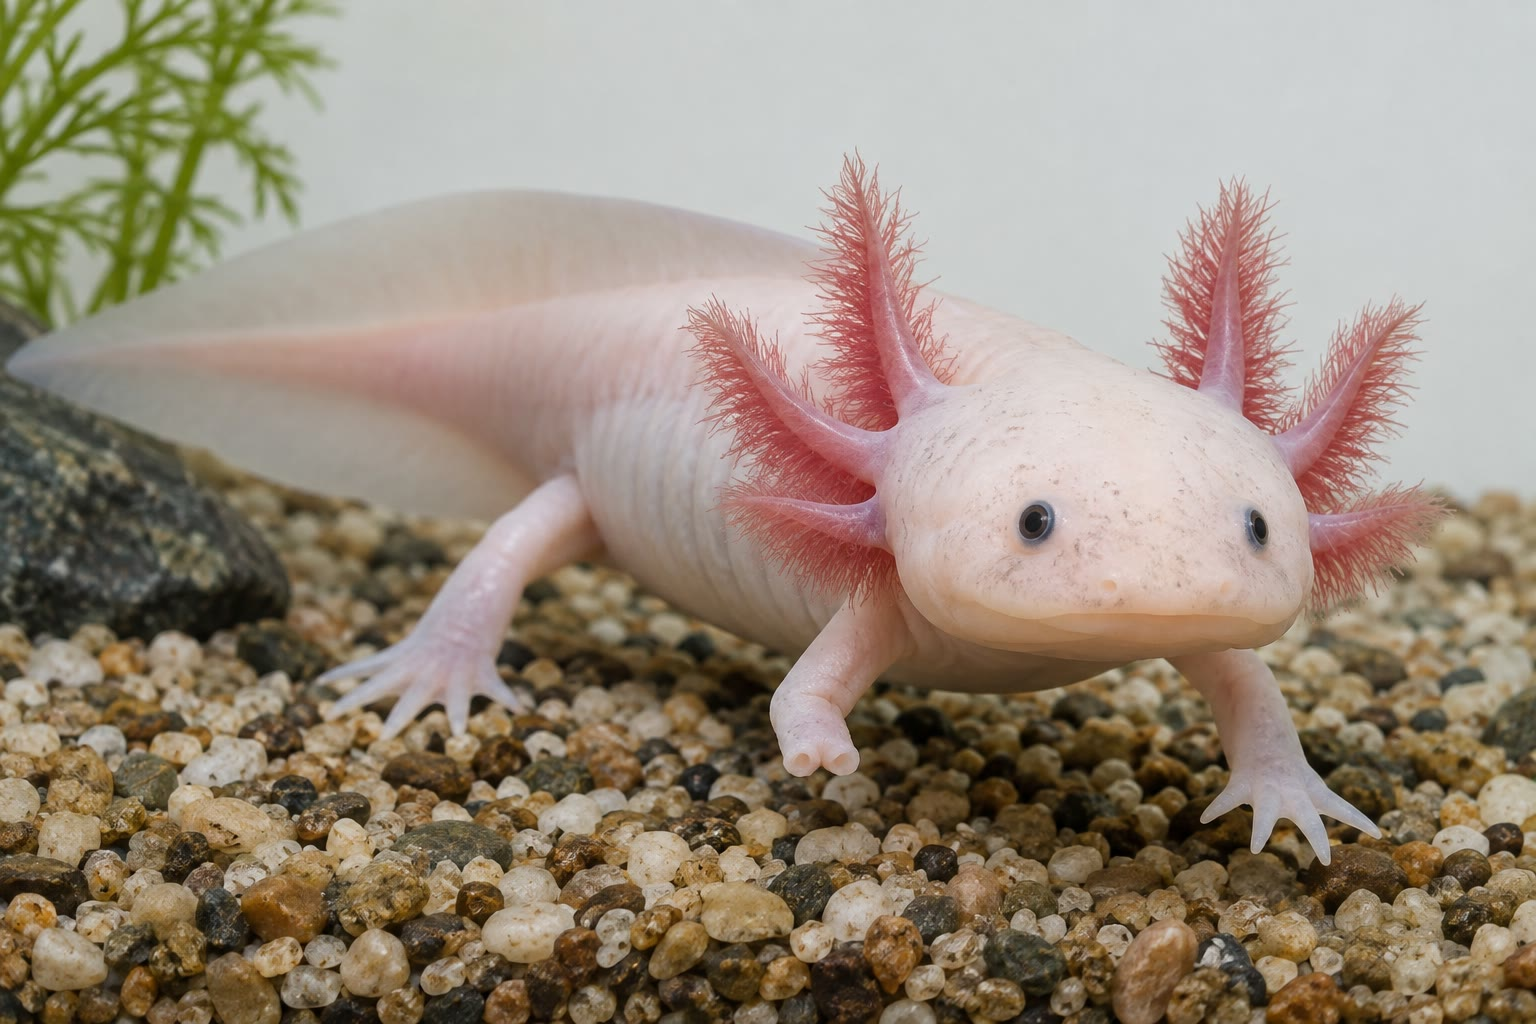
\includegraphics[width=0.46\linewidth]{images/book5/ai/b5-24-axolotl.jpg}\hspace{0.04\linewidth}
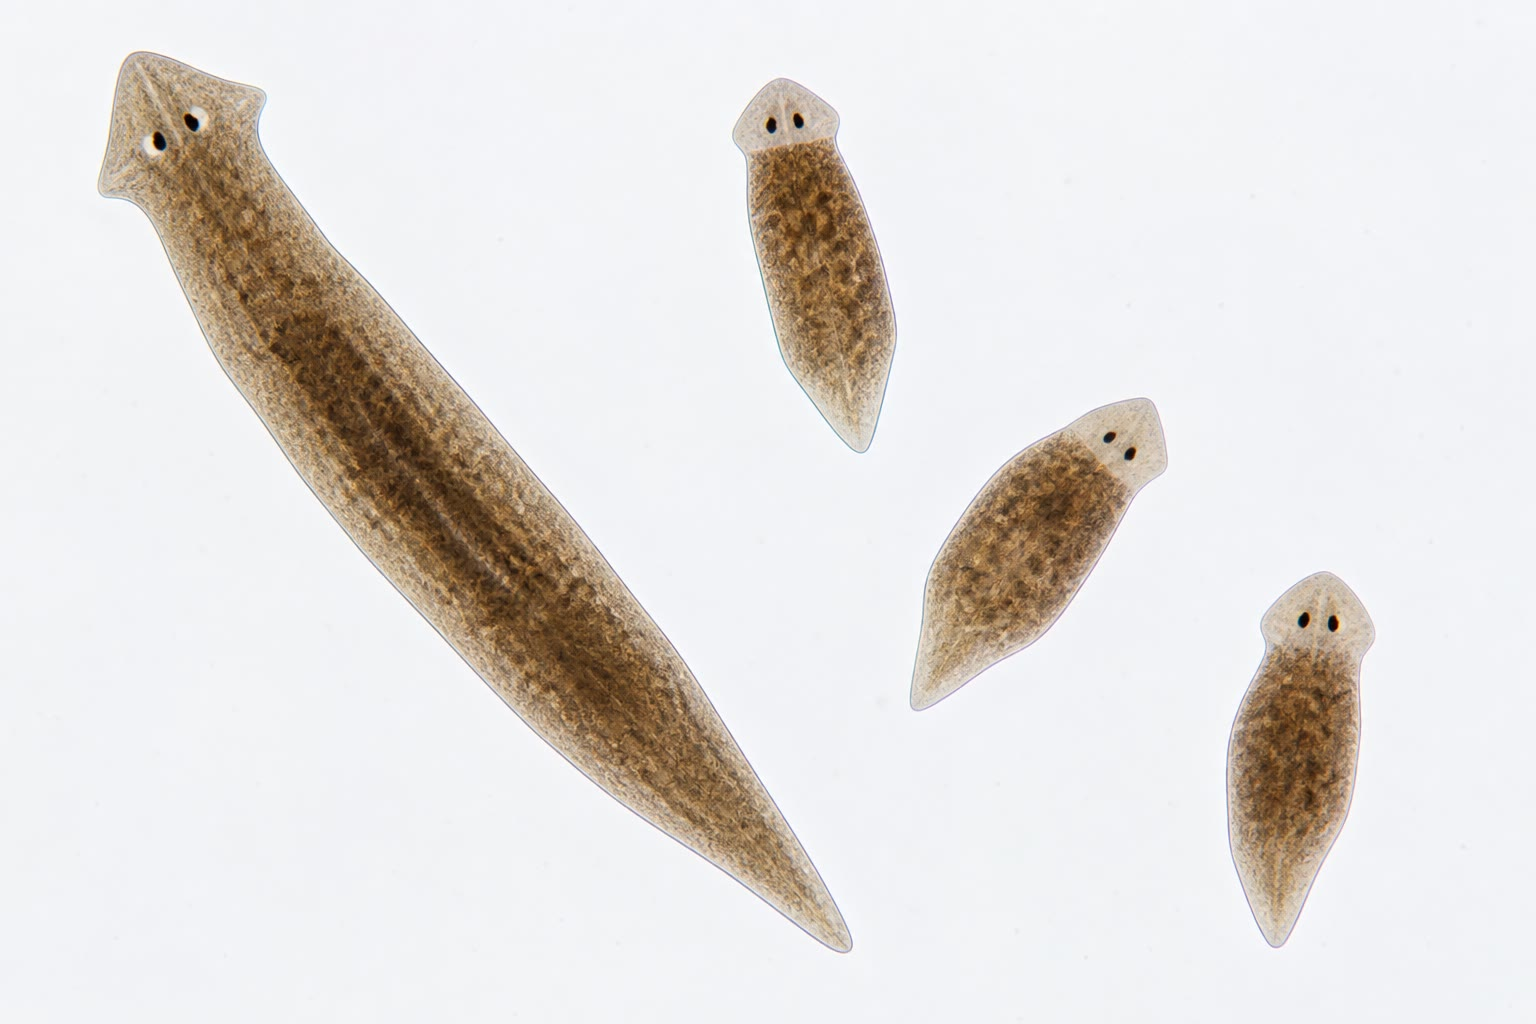
\includegraphics[width=0.46\linewidth]{images/book5/ai/b5-24-planarian-regeneration.jpg}

{\small Links: een axolotl, die in twee maanden een ledemaat laat
teruggroeien uit een \omterm{def:b3:stem-cells:regeneration}{blasteem} van gededifferentieerde cellen en dat
zijn hele leven kan blijven doen. Rechts: een planarie in stukken
gesneden, waarbij elk stuk binnen twee weken uit zijn \omterm{def:b3:stem-cells:regeneration}{neoblasten} een
complete worm laat teruggroeien.}
\end{omfigure}

\begin{proof}[Bewijsmateriaal]
Morgan (1898) sneed planariën in 279 stukken en vond dat elk een hele
worm liet teruggroeien tot een ondergrens van ongeveer een honderdste
van het lichaam; Reddien en collega's (2011) plaatsten één \omterm{def:b3:stem-cells:regeneration}{neoblast} in
een dodelijk bestraalde worm en herstelden die volledig --- één cel,
elk weefsel. Kragl en collega's (2009) maakten axolotls waarvan telkens
één weefsel groen was gemerkt en plaatsten die in ongemerkte
gastheren: na amputatie leverde groene spier alleen spier op en groen
kraakbeen alleen kraakbeen --- het \omterm{def:b3:stem-cells:regeneration}{blasteem} is geen poel van
pluripotente cellen maar een verzameling \omterm{def:b3:stem-cells:stem}{voorlopercellen} die tot hun
eigen lijn beperkt zijn, elk niet verder gededifferentieerd dan tot de
voorloper van het eigen weefsel. Singer (1952) liet zien dat een
ledemaat van een salamander alleen regenereert als er een drempelaantal
zenuwvezels de stomp bereikt, en dat een zenuw omleiden naar een wond
op de flank daar een ledemaat deed groeien.
\end{proof}

\section{De rekenkunde van de veroudering}

\begin{theorem}[Telomeren en de limiet van Hayflick]\label{thm:b3:stem-cells:hayflick}
\index{telomeer}\index{limiet van Hayflick}\index{eindreplicatieprobleem}\index{telomerase}\index{replicatieve veroudering}
Elk chromosoom eindigt in een \emph{telomeer}, enkele kilobasen van de
herhaling TTAGGG. Omdat het DNA-polymerase het laatste stuk van de
achterblijvende streng niet kan voltooien (het
\emph{eindreplicatieprobleem}), verkort elke deling elk telomeer met
$\Delta \approx$ \qtyrange{50}{100}{bp}. Uitgaande van
$L_{0} \approx \qty{10}{kb}$ en met een \emph{\omterm{thm:b3:stem-cells:hayflick}{replicatieve veroudering}}
--- een blijvende, door p53 afgedwongen stilstand --- die intreedt
zodra het kortste telomeer $L_{\text{crit}} \approx \qty{4}{kb}$
bereikt, kan een cellijn hoogstens
\[
n_{\max} = \frac{L_{0} - L_{\text{crit}}}{\Delta} \approx \frac{6000}{50\text{--}100} \approx 60\text{--}120
\]
maal delen: de \emph{\omterm{thm:b3:stem-cells:hayflick}{limiet van Hayflick}}, de ruim vijftig
populatieverdubbelingen die menselijke fibroblasten in kweek voltooien
voordat zij stoppen. Het enzym \emph{\omterm{def:b3:cancer-biology:telomerase}{telomerase}}, een reverse
transcriptase met een RNA-sjabloon, verlengt de uiteinden weer; het is
werkzaam in de kiembaan, in embryonale en vele volwassen \omterm{def:b3:stem-cells:stem}{stamcellen}, en
in \qty{90}{\%} van de \omterm{def:b3:cancer-biology:hallmarks}{kankers}, die aan de limiet zijn ontsnapt door
het weer aan te zetten. Een \omterm{def:b3:stem-cells:stem}{stamcel} die $d$ maal per jaar deelt en wier
\omterm{def:b3:cancer-biology:telomerase}{telomerase} een deel $f$ van het verlies goedmaakt, heeft
$n_{\max} = (L_{0} - L_{\text{crit}})/[(1 - f)\Delta]$ delingen, en een
levensduur van $n_{\max}/d$ jaar: met $f = 0.7$, $\Delta
= 60$ en $d = 1$ zo'n 330 jaar voor een bloedvormende \omterm{def:b3:stem-cells:stem}{stamcel} --- maar
haar \omterm{def:b3:stem-cells:stem}{voorlopercellen}, met \omterm{def:b3:cancer-biology:telomerase}{telomerase} uit en twintig delingen tot een
rode cel, besteden bij elke lijn een vijfde van hun reserve, en daarom
hebben de bloedcellen van oude mensen kortere telomeren dan die van
jonge, met ongeveer \qty{30}{bp} per jaar.
\end{theorem}
\begin{proof}
Het verlies per deling is een vaste lengte, dus daalt de lengte van het
telomeer lineair met het aantal delingen, $L_{n} = L_{0} - n\Delta$, en
bereikt zij $L_{\text{crit}}$ bij $n = (L_{0} - L_{\text{crit}})/\Delta$;
met gedeeltelijke compensatie is het netto verlies per deling
$(1 - f)\Delta$. Hayflick en Moorhead (1961) toonden aan dat normale
menselijke fibroblasten na ongeveer vijftig verdubbelingen stoppen,
welke kweekomstandigheden er ook heersen, dat cellen die na twintig
verdubbelingen worden ingevroren en later ontdooid alleen de resterende
dertig voltooien --- zij tellen delingen, geen tijd --- en dat de
limiet lager ligt voor cellen van oude donoren. Harley, Futcher en
Greider (1990) maten hoe telomeren korter werden met het aantal
verdubbelingen in kweek en met de leeftijd van de donor; Bodnar en
collega's (1998) brachten \omterm{def:b3:cancer-biology:telomerase}{telomerase} in normale cellen en die deelden
onbeperkt voorbij de limiet zonder kankerachtig te worden, waarmee het
telomeer als klok werd vastgesteld.
\end{proof}

\begin{omfigure}
\begin{tikzpicture}
\begin{axis}[
  width=0.62\linewidth, height=5.4cm,
  axis x line=bottom, axis y line=left,
  xmin=0, xmax=120, ymin=0, ymax=11,
  xlabel={populatieverdubbelingen}, ylabel={lengte van het telomeer (kb)},
  xlabel style={font=\small, at={(axis description cs:0.5,-0.12)}, anchor=north}, ylabel style={font=\small},
  tick label style={font=\small}, xtick={0,30,60,90,120}, ytick={4,7,10},
  clip=false,
]
\addplot[very thick, omDef, domain=0:60, samples=2] {10-0.1*x};
\addplot[very thick, omThm, domain=0:120, samples=2] {10-0.05*x};
\addplot[very thick, omMeth!70!black, domain=0:120, samples=2] {10-0.015*x};
\draw[dashed, gray] (axis cs:0,4) -- (axis cs:120,4); \node[font=\scriptsize, gray, anchor=north west] at (axis cs:2,3.9) {veroudering bij $L_{\text{crit}} = \qty{4}{kb}$};
\node[font=\scriptsize, omDef, anchor=south west] at (axis cs:63,4.3) {$\Delta = \qty{100}{bp}$: 60 verdubbelingen};
\node[font=\scriptsize, omThm, anchor=west] at (axis cs:70,8.0) {$\Delta = \qty{50}{bp}$: 120};
\node[font=\scriptsize, omMeth!70!black, anchor=south west, align=left] at (axis cs:78,9.3) {telomerase compenseert\\\qty{70}{\%}: 400};
\fill[omDef] (axis cs:60,4) circle (2pt); \fill[omThm] (axis cs:120,4) circle (2pt);
\end{axis}
\end{tikzpicture}

{\small Telomeren als teller van delingen. Een vast verlies per deling
geeft een rechte lijn; waar zij de kritieke lengte kruist houdt de lijn
op. \omterm{def:b3:cancer-biology:telomerase}{Telomerase} vlakt de helling af en heft de limiet, volledig
werkzaam, geheel op --- in de kiembaan, en in \omterm{def:b3:cancer-biology:hallmarks}{kankers}.}
\end{omfigure}

\begin{proposition}[De wet van Gompertz]\label{prop:b3:stem-cells:gompertz}
\index{wet van Gompertz}\index{sterftecijfer}\index{kenmerken van de veroudering}\index{verouderde cel}
Boven ongeveer dertig jaar verdubbelt het menselijke sterftecijfer
$\mu(t)$ --- de kans om in het komende jaar te sterven --- elke acht
jaar: $\mu(t) =
\mu_{0}\,\mathrm{e}^{\gamma(t - t_{0})}$ met $\gamma = \ln 2/8 \approx
\qty{0.087}{yr^{-1}}$ (Gompertz, 1825). De overleving tot leeftijd $t$ is dan
\[
S(t) = \exp\!\Bigl[-\frac{\mu_{0}}{\gamma}\bigl(\mathrm{e}^{\gamma(t - t_{0})} - 1\bigr)\Bigr],
\]
een kromme die decennialang vlak is en daarna steil daalt, met een
mediane levensduur
$t_{1/2} = t_{0} + \gamma^{-1}\ln(1 + \gamma\ln 2/\mu_{0})$: voor
$\mu_{0} = 10^{-3}$ per jaar op dertigjarige leeftijd ongeveer
$30 + 47 = 77$ jaar. Dezelfde wet geldt, met andere constanten, voor
muizen (verdubbelingstijd drie maanden), honden, vliegen en wormen:
veroudering is een exponentiële stijging van de kwetsbaarheid, geen
klok die afloopt. De biologie achter de exponent is een stel op elkaar
inwerkende \emph{kenmerken}: opgehoopte DNA-schade en epigenetische
drift, slijtage van de telomeren, verlies van de eiwithuishouding,
achteruitgang van de mitochondriën, uitputting van de voorraden
\omterm{def:b3:stem-cells:stem}{stamcellen}, de ophoping van \emph{verouderde cellen} die niet meer
delen maar ontstekingssignalen uitscheiden, en chronische \omterm{def:b3:innate-immunity:inflammation}{ontsteking};
bij muizen verlengt het opruimen van verouderde cellen of het beperken
van de calorieën het leven, en bij wormen verdubbelt één mutatie in de
insulineachtige route het. Of de exponent bij de mens kan worden
verlaagd, in plaats van de constante $\mu_{0}$ die de geneeskunde in
een eeuw tienvoudig heeft verkleind, is de open vraag.
\end{proposition}
\begin{proof}
Is $\mu$ het risico, dan geldt $\mathrm{d}S/\mathrm{d}t = -\mu(t)S$, dus $\ln S =
-\int_{t_{0}}^{t}\mu = -(\mu_{0}/\gamma)(\mathrm{e}^{\gamma(t-t_{0})} -
1)$. Stel $S = 1/2$: $\mathrm{e}^{\gamma(t-t_{0})} = 1 + \gamma\ln 2/
\mu_{0}$, waaruit de mediaan volgt; met $\gamma = 0.087$ en $\mu_{0} =
10^{-3}$ is $\ln(1 + 60) = 4.1$ en $t - t_{0} = 47$. De empirische wet
is de fit van Gompertz aan de Engelse sterftetafels; dat zij zoveel
soorten met een gedeelde vorm en soortspecifieke constanten beschrijft
wordt hier aangenomen als de samenvatting van een eeuw demografie.
\end{proof}

\begin{omfigure}
\begin{tikzpicture}
\begin{semilogyaxis}[
  width=0.5\linewidth, height=5.2cm,
  axis x line=bottom, axis y line=left,
  xmin=20, xmax=100, ymin=0.0003, ymax=1,
  xlabel={leeftijd (jaren)}, ylabel={sterftecijfer per jaar},
  xlabel style={font=\small, at={(axis description cs:0.5,-0.12)}, anchor=north}, ylabel style={font=\small},
  tick label style={font=\small}, xtick={30,50,70,90}, ytick={0.001,0.01,0.1,1}, yticklabels={0.001,0.01,0.1,1},
  clip=false,
]
\addplot[very thick, omDef, domain=30:100, samples=2] {0.001*exp(0.0866*(x-30))};
\node[font=\scriptsize, omDef, anchor=north west, align=left] at (axis cs:32,0.3) {$\mu = \mu_{0}\,\mathrm{e}^{\gamma(t-30)}$\\verdubbeling elke 8 jaar};
\end{semilogyaxis}
\begin{axis}[
  at={(0.55\linewidth,0)}, anchor=south west,
  width=0.43\linewidth, height=5.2cm,
  axis x line=bottom, axis y line=left,
  xmin=20, xmax=110, ymin=0, ymax=1.05,
  xlabel={leeftijd (jaren)}, ylabel={overlevend deel},
  xlabel style={font=\small, at={(axis description cs:0.5,-0.12)}, anchor=north}, ylabel style={font=\small},
  tick label style={font=\small}, xtick={30,50,77,100}, ytick={0.5,1},
  clip=false,
]
\addplot[very thick, omThm, domain=30:110, samples=80] {exp(-(0.001/0.0866)*(exp(0.0866*(x-30))-1))};
\draw[dashed, gray] (axis cs:77,0) -- (axis cs:77,0.5) -- (axis cs:20,0.5);
\node[font=\scriptsize, omThm, anchor=north east, align=right] at (axis cs:75,0.45) {mediaan\\77 jaar};
\end{axis}
\end{tikzpicture}

{\small De \omterm{prop:b3:stem-cells:gompertz}{wet van Gompertz}. Links: op een logaritmische as is het
sterftecijfer vanaf dertig jaar een rechte lijn. Rechts: de
overlevingskromme die daaruit volgt --- een plateau en dan een klif,
met de mediaan waar de integraal van het risico $\ln 2$ bereikt.}
\end{omfigure}

\begin{remark}[Vernieuwing en haar prijs]\label{rem:b3:stem-cells:remark}
Een lichaam dat zichzelf vernieuwt moet cellen houden die onbeperkt
kunnen delen, en cellen die onbeperkt kunnen delen zijn de grondstof
van \omterm{def:b3:cancer-biology:hallmarks}{kanker}; een lichaam dat zich tegen \omterm{def:b3:cancer-biology:hallmarks}{kanker} beschermt door delingen
te tellen en veroudering af te dwingen moet op den duur te weinig
cellen overhouden die kunnen delen. De hiërarchie van de \omterm{def:b3:stem-cells:stem}{stamcellen} is
één oplossing --- weinig trage cellen beschermd in nissen, veel snelle
cellen die spoedig sterven --- en de \omterm{thm:b3:stem-cells:hayflick}{limiet van Hayflick} een andere, en
de e-macht van Gompertz is de som van hun kosten. De salamander betaalt
anders: hij verdraagt cellen die dedifferentiëren en laat een poot
teruggroeien, en hij is koudbloedig, traag en leeft zelden lang genoeg
om de rekening van de \omterm{def:b3:cancer-biology:hallmarks}{kanker} te betalen. De cellen waarmee een mens is
geboren zijn grotendeels niet de cellen die hij heeft; de cellen die de
vervangers maakten zijn de cellen die hij moet behouden.
\end{remark}

\section{Opgaven}

\begin{exercise}[$\star$]\label{exo:b3:stem-cells:1}
Definieer \omterm{def:b3:stem-cells:stem}{zelfvernieuwing}, potentie, \omterm{def:b3:stem-cells:stem}{nis} en \omterm{def:b3:stem-cells:stem}{doorgangsversterkende cel},
en geef van elk een voorbeeld in de darm.
\end{exercise}

\begin{exercise}[$\star$]\label{exo:b3:stem-cells:2}
Wat toonde de proef met de miltkolonies aan, en welke eigenschap van
een \omterm{def:b3:stem-cells:stem}{stamcel} vergde een tweede muis om te worden aangetoond?
\end{exercise}

\begin{exercise}[$\star$]\label{exo:b3:stem-cells:3}
Noem de vier factoren van Yamanaka en leg uit waarom het
herprogrammeren weken duurt en bij één op de duizend cellen slaagt.
\end{exercise}

\begin{exercise}[$\star$]\label{exo:b3:stem-cells:4}
Zet de wegen naar \omterm{def:b3:stem-cells:regeneration}{regeneratie} van de planarie en van de salamander
tegenover elkaar, en zeg wat de transplantaties van Kragl over het
\omterm{def:b3:stem-cells:regeneration}{blasteem} lieten zien.
\end{exercise}

\begin{exercise}[$\star\star$]\label{exo:b3:stem-cells:5}
Telomeren beginnen op \qty{11}{kb}, de veroudering treedt in bij
\qty{5}{kb}, het verlies is \qty{75}{bp} per deling. \omterm{thm:b3:stem-cells:hayflick}{Limiet van
Hayflick}? Cellen van een donor van 70 jaar hebben \qty{8}{kb}: hoeveel
verdubbelingen resten er? Als \omterm{def:b3:cancer-biology:telomerase}{telomerase} \qty{60}{\%} van het verlies
goedmaakt, wat is dan de limiet?
\end{exercise}

\begin{exercise}[$\star\star$]\label{exo:b3:stem-cells:6}
Een crypte bevat 14 \omterm{def:b3:stem-cells:stem}{stamcellen} die eens per dag delen en doorgangscellen
voeden die nog 4 maal delen, en de crypte levert haar villus \num{300}
cellen per dag. Controleer de rekenkunde: hoeveel delingen van
\omterm{def:b3:stem-cells:stem}{stamcellen} per dag leveren differentiërende dochters op, en met hoeveel
\omterm{def:b3:stem-cells:stem}{stamcellen} aan delingen komt dat overeen?
\end{exercise}

\begin{exercise}[$\star\star$]\label{exo:b3:stem-cells:7}
Het lichaam maakt $2\times 10^{11}$ rode cellen per dag, elk het
resultaat van ongeveer 20 delingen vanaf een \omterm{def:b3:stem-cells:stem}{stamcel}. Hoeveel delingen
van \omterm{def:b3:stem-cells:stem}{stamcellen} per dag vergt dat, en hoe vaak deelt elk van de
\num{10000} \omterm{def:b3:stem-cells:stem}{stamcellen} dan? Vergelijk met de waargenomen ``ongeveer
eens per jaar'' en verklaar het verschil.
\end{exercise}

\begin{exercise}[$\star\star$]\label{exo:b3:stem-cells:8}
Bereken met $\gamma = \qty{0.087}{yr^{-1}}$ en $\mu_{0} = 10^{-3}$ op
dertigjarige leeftijd het sterftecijfer op 50, 70 en 90 jaar, de
overleving tot 70 en 90, en de mediane levensduur. Wat doet het
halveren van $\mu_{0}$ met de mediaan? En het halveren van $\gamma$?
\end{exercise}

\begin{exercise}[$\star\star$]\label{exo:b3:stem-cells:9}
Twee derde van de lever van een rat wordt weggenomen. De overgebleven
levercellen, die alle delen, herstellen de massa in tien dagen. Hoeveel
delingen heeft elk nodig? Waarom heet dit \omterm{def:b3:stem-cells:regeneration}{compenserende groei} en geen
\omterm{def:b3:stem-cells:regeneration}{regeneratie}, en wat bouwt de lever \emph{niet} opnieuw op?
\end{exercise}

\begin{exercise}[$\star\star\star$]\label{exo:b3:stem-cells:10}
\omterm{prop:b3:stem-cells:crypt}{Neutrale drift}: $N$ \omterm{def:b3:stem-cells:stem}{stamcellen} in een \omterm{def:b3:stem-cells:stem}{nis} delen symmetrisch; bij elke
gebeurtenis deelt er één cel en gaat er één willekeurig verloren, zodat
het aantal van een gegeven kloon een toevalswandeling tussen $0$ en $N$
maakt. Beredeneer dat de kans dat een kloon van $k$ cellen de \omterm{def:b3:stem-cells:stem}{nis}
uiteindelijk overneemt gelijk is aan $k/N$, en dat een kloon van één
cel bij $N = 14$ een kans van $1/14$ heeft. Wat voorspelt dit voor het
lot van een \omterm{def:b3:stem-cells:stem}{stamcel} met een nieuwe neutrale mutatie?
\end{exercise}

\begin{exercise}[$\star\star\star$]\label{exo:b3:stem-cells:11}
Een mutatie geeft een kloon \omterm{def:b3:stem-cells:stem}{stamcellen} een voordeel van \qty{10}{\%} in
de mededinging van \cref{exo:b3:stem-cells:10}. Leg in grote lijnen uit
waarom haar kans op overname ruim boven $k/N$ stijgt, waarom de crypten
en het merg van oude mensen steeds meer door enkele klonen worden
beheerst (klonale hematopoëse), en waarom dat een eerste stap naar
\omterm{def:b3:cancer-biology:hallmarks}{kanker} is zonder \omterm{def:b3:cancer-biology:hallmarks}{kanker} te zijn.
\end{exercise}

\begin{exercise}[$\star\star\star$]\label{exo:b3:stem-cells:12}
Stel dat de exponent $\gamma$ van Gompertz een tempo van opstapelende
schade weerspiegelt en de constante $\mu_{0}$ de omgeving. De
geneeskunde heeft $\mu_{0}$ sinds 1900 tienvoudig verkleind zonder
$\gamma$ te veranderen. Bereken de winst in mediane levensduur die die
tienvoudige verlaging geeft, en de verdere winst van nog een
tienvoudige verlaging; leg uit waarom de opbrengst afneemt, en wat een
verlaging van $\gamma$ met \qty{20}{\%} in plaats daarvan zou doen.
\end{exercise}

\section{Vraagstuk: de cellen van bij de geboorte}

\begin{problem}[{Weekendvraagstuk --- de vernieuwing van een lichaam in
getallen: de hiërarchie van het bloed en wat zij van haar stamcellen
vraagt, de drift in de crypte, de telomeerklok en hoe telomerase en
voorlopercellen haar besteden, de kromme van Gompertz voor de
bevolking, en de afwegingen die een regenererend dier aanvaardt,
eindigend bij het aantal van Hayflick, de levensreserve van de stamcel
en de mediane levensduur}]
\label{pb:b3:stem-cells:1}
Gegevens: rode cellen $2.5\times 10^{11}$ per dag, granulocyten
$10^{11}$ per dag; $20$ delingen van \omterm{def:b3:stem-cells:stem}{stamcel} tot rijpe cel; \num{10000}
bloedvormende \omterm{def:b3:stem-cells:stem}{stamcellen}. Telomeren: $L_{0} = \qty{10}{kb}$,
$L_{\text{crit}} = \qty{4}{kb}$, $\Delta = \qty{60}{bp}$ per deling;
het \omterm{def:b3:cancer-biology:telomerase}{telomerase} in \omterm{def:b3:stem-cells:stem}{stamcellen} maakt $f = 0.7$ goed, dat in
\omterm{def:b3:stem-cells:stem}{voorlopercellen} niets. Crypte: $N = 14$ \omterm{def:b3:stem-cells:stem}{stamcellen}, één deling per dag.
Gompertz: $\mu_{0} =
10^{-3}$ per jaar op 30-jarige leeftijd, $\gamma = \qty{0.087}{yr^{-1}}$.
Ledemaat van een axolotl: \qty{40}{mm} teruggegroeid in \qty{60}{dagen};
een \omterm{def:b3:stem-cells:regeneration}{blasteem} van $10^{5}$ cellen dat tot $10^{8}$ groeit.

\medskip
\noindent\textbf{Deel I --- Het bloed.}
\begin{enumerate}
  \item Het aantal cellen dat per dag in totaal wordt gemaakt, en per seconde.
  \item Elke rijpe cel is het einde van $20$ delingen: hoeveel cellen
        levert één vastgelegde dochter van een \omterm{def:b3:stem-cells:stem}{stamcel} op? Hoeveel
        vastgelegde dochters per dag zijn er nodig?
  \item Hoeveel differentiërende delingen per \omterm{def:b3:stem-cells:stem}{stamcel} per dag betekent
        dat met \num{10000} \omterm{def:b3:stem-cells:stem}{stamcellen}? En per jaar?
  \item De gemeten deling van \omterm{def:b3:stem-cells:stem}{stamcellen} is ongeveer eens per jaar.
        Breng dat in overeenstemming: wat moeten de \omterm{def:b3:stem-cells:stem}{voorlopercellen}
        doen wat de berekening van vraag~3 aan de \omterm{def:b3:stem-cells:stem}{stamcellen} toeschreef?
  \item \omterm{def:b3:stem-cells:stem}{Voorlopercellen} hebben geen \omterm{def:b3:cancer-biology:telomerase}{telomerase}. Welke telomeerlengte
        bereikt een voorloper van een rode cel na haar $20$ delingen,
        uitgaande van \qty{10}{kb}? Maakt het uit dat die boven
        $L_{\text{crit}}$ ligt?
  \item Een \omterm{def:b3:stem-cells:stem}{stamcel} die eens per jaar deelt met $f = 0.7$: het netto
        verlies per deling, de delingen tot veroudering, en de jaren.
        Geef commentaar.
\end{enumerate}

\medskip
\noindent\textbf{Deel II --- De crypte.}
\begin{enumerate}[resume]
  \item Delingen per crypte per dag op de laag van de \omterm{def:b3:stem-cells:stem}{stamcellen}; als
        de helft van de gebeurtenissen een verloren \omterm{def:b3:stem-cells:stem}{stamcel} vervangt en
        de helft de doorgangszone voedt, hoeveel vastgelegde cellen per
        dag, en hoeveel villuscellen na $4$ doorgangsdelingen?
  \item De kans op overname van een kloon van één cel is $1/N$. De
        verwachte tijd tot eenkleurigheid is van de orde $N^{2}$
        delingsgebeurtenissen per cel; schat die in dagen en vergelijk
        met de waarnemingen met confetti (maanden).
  \item Een \omterm{def:b3:stem-cells:stem}{stamcel} verwerft een mutatie. Wat is de kans dat zij
        uiteindelijk in haar crypte wordt vastgelegd? In hoeveel van de
        $10^{7}$ crypten van een dikke darm zou een mutatie die eens
        per crypte ontstaat worden vastgelegd?
  \item Waarom beschermt de drift in een crypte beter tegen \omterm{def:b3:cancer-biology:hallmarks}{kanker} dan
        een weefsel waarin elke \omterm{def:b3:stem-cells:stem}{stamcel} levenslang asymmetrisch deelt?
  \item Nadat bestraling de \omterm{def:b3:stem-cells:stem}{stamcellen} heeft gedood keren doorgangscellen
        terug en vullen zij de \omterm{def:b3:stem-cells:stem}{nis} opnieuw. Wat zegt dat over waar de
        stamcelaard huist?
  \item Schets het lijnvolgexperiment dat symmetrische drift van
        \omterm{def:b3:stem-cells:stem}{asymmetrische deling} onderscheidt, en de twee uitkomsten.
\end{enumerate}

\medskip
\noindent\textbf{Deel III --- De klok.}
\begin{enumerate}[resume]
  \item De \omterm{thm:b3:stem-cells:hayflick}{limiet van Hayflick} voor een somatische lijn zonder \omterm{def:b3:cancer-biology:telomerase}{telomerase}.
  \item Een kweek fibroblasten wordt na $25$ verdubbelingen ingevroren
        en tien jaar later ontdooid: hoeveel verdubbelingen resten er?
        Wat toont dat over wat de cel telt?
  \item Telomeren van leukocyten worden bij volwassenen \qty{30}{bp}
        per jaar korter. Wanneer zouden zij vanaf \qty{8}{kb} op
        twintigjarige leeftijd $L_{\text{crit}}$ bereiken? Vergelijk
        met de levensduur en geef commentaar.
  \item \omterm{def:b3:cancer-biology:telomerase}{Telomerase} in normale fibroblasten laat hen de limiet passeren
        zonder kankerachtig te worden. \omterm{def:b3:cancer-biology:telomerase}{Telomerase} is werkzaam in
        \qty{90}{\%} van de \omterm{def:b3:cancer-biology:hallmarks}{kankers}. Breng die twee uitspraken met
        elkaar in overeenstemming.
  \item Bereken het sterftecijfer van Gompertz op 40, 60, 80 en 100
        jaar, en de overleving tot elk.
  \item De mediane levensduur; en de leeftijd waarop \qty{10}{\%} nog leeft.
\end{enumerate}

\medskip
\noindent\textbf{Deel IV --- Teruggroeien.}
\begin{enumerate}[resume]
  \item Axolotl: het gemiddelde tempo van teruggroei in mm/dag; het
        aantal verdubbelingen waarmee het \omterm{def:b3:stem-cells:regeneration}{blasteem} van $10^{5}$ tot
        $10^{8}$ cellen groeit, en de gemiddelde verdubbelingstijd over
        60 dagen.
  \item Als gededifferentieerde cellen hun leven lang delen zoals die
        van het \omterm{def:b3:stem-cells:regeneration}{blasteem} en een deling per cel een kans van $10^{-9}$
        op een oncogene mutatie draagt, hoeveel van zulke mutaties
        ontstaan er dan bij één \omterm{def:b3:stem-cells:regeneration}{regeneratie}? Waarom krijgt de axolotl
        toch bijna nooit \omterm{def:b3:cancer-biology:hallmarks}{kanker}, en waarom zou een zoogdier daar niet
        mee wegkomen?
  \item De zenuwen uit de stomp halen stopt de \omterm{def:b3:stem-cells:regeneration}{regeneratie}. Stel een
        experiment voor dat laat zien dat de zenuw een diffundeerbare
        stof levert, en één mogelijke identiteit van die stof.
  \item Een staartstuk van een planarie laat een tweede staart in
        plaats van een kop groeien wanneer een remmer van Wnt wordt
        uitgeschakeld. Verklaar dat met een gradiënt en met het
        positiegeheugen van het stuk.
  \item Een menselijke lever na een resectie van twee derde: welk deel
        van de levercellen moet één maal delen, welk deel tweemaal, om
        de massa te herstellen? Waarom is het resultaat een werkende
        lever met de verkeerde vorm?
  \item Waarom zou een lichaam dat als een axolotl regenereerde een
        andere kromme van Gompertz hebben, en welke kant op?
  \item Vat samen: het aantal van Hayflick (vraag~13), de delingen en
        jaren van een \omterm{def:b3:stem-cells:stem}{stamcel} met hulp van \omterm{def:b3:cancer-biology:telomerase}{telomerase} (vraag~6), en de
        mediane levensduur (vraag~18).
\end{enumerate}
\end{problem}
